\documentclass[vi]{uet-awesome-thesis} % use [vi] for vietnamese
\usepackage{tabularray}
\usepackage[linesnumbered]{algorithm2e}
\usepackage{tcolorbox}
\usepackage{float}



\title{\Large Cải thiện hiệu năng thuật toán phát hiện bất thường MIDAS-R trong an ninh mạng}
\author{Nguyễn Lê Việt Hoàng}
\major{Điện Tử Viễn Thông}
\advisor{Prof. Nguyễn Nam Hoàng}
\university{University of Engineering and Technology}
\universitycity{Hanoi}
\degreeyear{2023}
\renewcommand{\glsmcols}{2}
\setglossarystyle{mcolindex}

\newacronym{wsn}{WSN}{wireless sensor network}
\newacronym{wrsn}{WRSN}{wireless rechargeable sensor network}
\newacronym{qos}{QoS}{Quality of Service}
\newacronym{ia}{IA}{intelligent agent}
\newacronym{rl}{RL}{reinforcement learning}
\newacronym{dl}{DL}{deep learning}
\newacronym{mdp}{MDP}{Markov decision process}



\newglossary[nlg]{notation}{not}{ntn}{Notation}

\newglossaryentry{not:eth}{
    name=\ensuremath{\tilde{E}_{td}},
    description={energy requesting threshold},
    type=notation}
    
\newglossaryentry{not:bs}{
    name=\ensuremath{p_0},
    description={base station},
    type=notation}
    
\newglossaryentry{not:snset}{
    name=\ensuremath{\mathcal{P}},
    description={a set of deployed sensors},
    type=notation}

\newglossaryentry{not:num:sn}{
    name=\ensuremath{n},
    description={number of deployed sensors},
    type=notation}
    
\newglossaryentry{not:sn}{
    name=\ensuremath{p},
    description={a sensor},
    type=notation}
    

\makeglossaries 

\begin{document}

%%%%%%%%%%%%%%%%%%%%%%%%%%%%%%%%
%title 
%%%%%%%%%%%%%%%%%%%%%%%%%%%%%%%%
\maketitle
% 
\makesidecover

\authorship

\approval
\pagenumbering{roman}

\acknowledgments{


And above all, this thesis is for Huong, the one that completes me.
}

\addcontentsline{toc}{chapter}{Abstract}
\abstractpage{
\setlength{\headheight}{15.59995pt}


\begin{center}
    \vspace*{1pt}
{\fontsize{13pt}{1}\textbf{TÓM TẮT}}
\end{center}



}

\tableofcontents
\addcontentsline{toc}{chapter}{List of Figures}
\listoffigures
\addcontentsline{toc}{chapter}{List of Tables}
\listoftables

\glsaddall
\printglossary[type=\acronymtype,title=List of Acronyms, toctitle=List of Acronyms]
\printglossary[type=notation,title=List of Notations, toctitle=List of Notations,nonumberlist]

\newpage
\pagenumbering{arabic}

\chapter{TỔNG QUAN}

Chương này nêu định nghĩa về ngành an ninh mạng,
đánh giá thực trạng về an toàn không gian mạng hiện nay và
khảo sát các phương pháp được sử dụng trong IDS( Intrusion Detection System)
để phát hiện các cuộc tấn công mạng.

\section{Giới thiệu về an ninh mạng}

An ninh mạng là một tập hợp các quy tắc và cấu hình được thiết kế để
bảo vệ tính toàn vẹn, bảo mật và khả năng truy cập của mạng máy tính
và dữ liệu bằng cả công nghệ phần mềm và phần cứng. Ngành an ninh mạng
đang phát triển nhanh chóng do nhu cầu ngày càng tăng đối với các giải
pháp và dịch vụ có thể ngăn chặn, phát hiện và giảm thiểu các cuộc tấn
công mạng vào các doanh nghiệp, cơ quan chính phủ và cá nhân. Theo nghiên cứu ---
Các yếu tố chính thúc đẩy sự tăng trưởng của thị trường bao gồm số lượng các
mối đe dọa mạng ngày càng tăng, việc áp dụng công nghệ đám mây và di
động và nhu cầu làm việc từ xa an toàn.


\section{Thực trạng an ninh mạng hiện nay}

Theo báo cáo của AAG\cite{survey2023} năm 2023,
bối cảnh an ninh mạng toàn cầu đã chứng kiến các mối đe
dọa gia tăng trong những năm gần đây. Trong đại dịch,
tội phạm mạng đã lợi dụng các mạng bị sai lệch khi các
doanh nghiệp chuyển sang môi trường làm việc từ xa.
Năm 2020, các cuộc tấn công bằng phần mềm độc hại tăng 358\% so
với năm 2019.

Từ đây, các cuộc tấn công mạng trên toàn cầu đã tăng 125\% cho
đến năm 2021 và số lượng các cuộc tấn công mạng ngày càng tăng
tiếp tục đe dọa các doanh nghiệp và cá nhân vào năm 2022.

Dưới đây là một số thông tin đáng chú ý:

\begin{itemize}
    \item Lừa đảo(Phishing) vẫn là hình thức phổ biến nhất của tội phạm trực tuyến. Vào năm 2021, 323.972 người dùng internet được cho là nạn nhân của các cuộc tấn công lừa đảo. Điều này có nghĩa là một nửa số người dùng bị vi phạm dữ liệu đã rơi vào một cuộc tấn công lừa đảo.
    \item Gần 1 tỷ email đã bị lộ trong một năm, ảnh hưởng đến 1/5 người dùng internet.
    \item Vi phạm dữ liệu khiến các doanh nghiệp thiệt hại trung bình 4,35 triệu đô la vào năm 2022.
    \item Khoảng 236,1 triệu cuộc tấn công ransomware đã xảy ra trên toàn cầu trong nửa đầu năm 2022.
    \item Cứ 2 người dùng internet ở Mỹ thì có 1 người bị xâm phạm tài khoản vào năm 2021.
    \item 39\% doanh nghiệp ở Vương quốc Anh cho biết đã bị tấn công mạng vào năm 2022.
    \item Khoảng 1 trong 10 tổ chức của Hoa Kỳ không có bảo hiểm chống lại các cuộc tấn công mạng.
    \item 53,35 Công dân Hoa Kỳ bị ảnh hưởng bởi tội phạm mạng trong nửa đầu năm 2022.
    \item Tội phạm mạng khiến các doanh nghiệp ở Vương quốc Anh thiệt hại trung bình £4200 vào năm 2022.
    \item Năm 2020, các cuộc tấn công bằng phần mềm độc hại đã tăng 358\% so với năm 2019.
\end{itemize}

\section{IDS và các phương pháp phát hiện tấn công}
% create sub section
\subsection{IDS - Intrusion Detection System}

Hệ thống phát hiện xâm nhập (IDS) là một ứng dụng phần mềm giám sát
các hoạt động của mạng hoặc hệ thống và phân tích chúng để tìm các
dấu hiệu vi phạm chính sách, cách sử dụng được chấp nhận hoặc các biện
pháp bảo mật tiêu chuẩn. Sau đó, nó sẽ báo cáo mọi hoạt động độc hại
hoặc vi phạm chính sách cho quản trị viên hệ thống. IDS có thể giúp
bảo vệ một tổ chức khỏi các cuộc tấn công mạng bằng cách phát hiện và
cảnh báo về các mối đe dọa tiềm ẩn trước khi chúng gây ra thiệt hại.

\subsection{Các phương pháp phát hiện tấn công trong IDS}

Có thể phân loại các IDS theo phương pháp phát hiện như sau:
\begin{itemize}
    \item IDS dựa trên chữ ký (SIDS) - Signature-based IDS:
          Hệ thống phát hiện xâm nhập chữ ký (SIDS) dựa trên
          về các kỹ thuật khớp mẫu để tìm ra một cuộc tấn công đã biết;
          chúng còn được gọi là Phát hiện dựa trên tri thức - Knowledge-based Detection(\cite{sids}).
          Trong SIDS, các phương thức đối sánh được sử dụng để tìm ra sự xâm nhập trước đó.
          Nói cách khác, khi một chữ ký xâm nhập phù hợp với
          chữ ký của một lần xâm nhập trước đó đã tồn tại
          trong cơ sở dữ liệu chữ ký, tín hiệu báo động được kích hoạt.
          Đối với SIDS, nhật ký của máy chủ được kiểm tra để tìm chuỗi
          các lệnh hoặc hành động trước đây đã được xác định là phần mềm độc hại.

    \item IDS dựa trên sự bất thường (AIDS) - Anomaly-based IDS:
          AIDS đã thu hút sự quan tâm của rất nhiều học giả do nó
          khả năng khắc phục hạn chế của SIDS. Trong AIDS, một
          mô hình bình thường của hành vi của một hệ thống máy tính là
          được tạo bằng cách sử dụng máy học(machine learing), dựa trên thống kê(statistical-based) hoặc
          phương pháp dựa trên tri thức(knowledge-based). Bất kỳ sai lệch đáng kể nào giữa hành vi được quan sát và mô hình đều được coi là
          như một sự bất thường, có thể được hiểu là một sự xâm nhập(intrusion).
          Giả định cho nhóm kỹ thuật này là hành vi ác ý khác với hành vi thông thường của người dùng. Các
          hành vi của người dùng bất thường không giống với
          các hành vi tiêu chuẩn được phân loại là xâm nhập. Sự phát triển của AIDS bao gồm hai giai đoạn: giai đoạn đào tạo
          và giai đoạn thử nghiệm. Trong giai đoạn đào tạo, bình thường
          hồ sơ lưu lượng truy cập được sử dụng để tìm hiểu một mô hình hành vi bình thường và sau đó trong giai đoạn thử nghiệm, một bộ dữ liệu mới được sử dụng
          để thiết lập khả năng khái quát hóa của hệ thống đối với các cuộc xâm nhập chưa từng thấy trước đây. AIDS có thể được phân loại thành một
          số loại dựa trên phương pháp được sử dụng cho
          đào tạo, ví dụ, dựa trên thống kê, dựa trên tri thức
          và dựa trên máy học\cite{aids}

\end{itemize}

Mỗi phương pháp đều có những ưu và nhược điểm riêng, điều này được tóm
gọn trong bảng dưới đây:

\definecolor{MineShaft}{rgb}{0.2,0.2,0.2}
\begin{table}[hbt!]
    \centering
    \caption{So sánh các phương pháp phát hiện tấn công trong IDS}
    \begin{tblr}{
        width = \linewidth,
        colspec = {Q[110]Q[70]Q[400]Q[596]},
        row{1} = {c},
        cell{2}{1} = {r=2}{c},
        cell{2}{2} = {c},
        cell{2}{3} = {t,fg=MineShaft},
        cell{2}{4} = {t,fg=MineShaft},
        cell{3}{2} = {c},
        cell{3}{3} = {t,fg=MineShaft},
        cell{3}{4} = {t,fg=MineShaft},
        vlines,
        hline{1-2,4} = {-}{},
                hline{3} = {2-4}{},
            }
        &  & \textbf{Ưu điểm} & \textbf{Nhược điểm}\\
        Phương pháp phát hiện & SIDS & {- Rất hiệu quả trong việc xác định xâm nhập với báo động sai tối thiểu (FA).\\- Phát hiện kịp thời các hành vi xâm nhập.\\- Vượt trội để phát hiện các cuộc tấn công đã biết.\\- Thiết kế đơn giản.} & {- Cần cập nhật chữ ký mới thường xuyên.\\- SIDS được thiết kế để phát hiện các cuộc tấn công đối với các chữ ký đã biết. Khi trước đó xâm nhập đã được thay đổi một chút thành một biến thể mới, thì hệ thống sẽ không thể xác định độ lệch mới này của cuộc tấn công tương tự.\\- Không thể phát hiện cuộc tấn công zero-day.\\- Không phù hợp để phát hiện các cuộc tấn công nhiều bước.\\- Ít hiểu biết sâu sắc về các cuộc tấn công}\\
        & AIDS & {- Có thể được sử dụng để phát hiện các cuộc tấn công mới.\\- Có thể được sử dụng để tạo chữ ký xâm nhập.} & {- AIDS không thể xử lý các gói được mã hóa, vì vậy cuộc tấn công có thể không bị phát hiện và có thể đưa ra một mối đe dọa.\\- Báo động dương tính giả cao.\\- Khó xây dựng một hồ sơ bình thường cho một hệ thống máy tính rất năng động.\\- Cảnh báo chưa được phân loại.\\- Cần đào tạo ban đầu.}
    \end{tblr}
\end{table}


Gần đây, một thuật toán phát hiện bất thường mới được đề xuất được gọi
là MIDAS hứa hẹn mang ưu điểm của cả hai nhóm trên đồng thời hạn chế nhược điểm của
các phương pháp được sử dụng trong AIDS.

\section{MIDAS - Microcluster-Based Detector of Anomalies in Edge Streams}
Phần này sẽ giới thiệu về  CMS, cấu trúc dữ liệu phác thảo được sử dụng
trong MIDAS. Tiếp đến là tổng quan về MIDAS và biến thể của nó, MIDAS-R. Cuối cùng là
đánh giá hiệu quả của chúng.

\subsection{Count-Min Sketch - Bản phác thảo đếm tối thiểu}
Câu hỏi đặt ra là: Cho một chuỗi dữ liệu liên tục,
làm thế nào để  biết số lần xuất hiện của một giá trị bất kỳ trong chuỗi đó?

CMS - Count-Min Sketch\cite{cms_full} là một cấu trúc dữ liệu trả lời câu hỏi trên với kích thước bộ nhớ cố định,
thời gian truy vấn không đổi và lưu trữ gần đúng số lần xuất hiện
của các giá trị trong chuỗi dữ liệu. Ý tưởng cơ bản của Count-Min Sketch khá đơn giản,
nó chỉ là một mảng hai chiều $(d \times w)$ của các bộ đếm số nguyên.
Khi một giá trị đến, nó được ánh xạ tới một vị trí tại mỗi $d$ hàng bằng cách sử dụng $d$ hàm
băm khác nhau. Bộ đếm trên mỗi vị trí được tăng lên. Quá trình này được thể hiện trong hình dưới đây:

% embedded image
\begin{figure}[h]
    \centering
    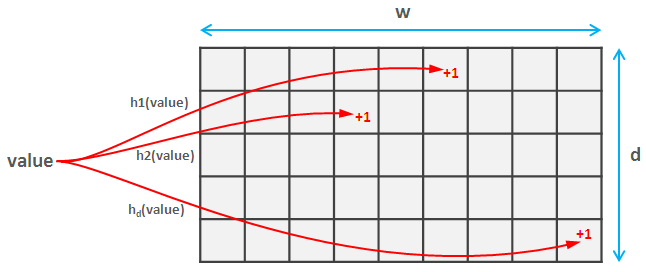
\includegraphics[width=1.0\textwidth]{figures/CMS.png}
    \caption{Minh họa Count-Min Sketch}
    \label{fig:1}
\end{figure}

Để truy vấn, ta chỉ cần trả về giá trị nhỏ nhất của các bộ đếm
tại các vị trí được ánh xạ tới giá trị đó.

Sự phụ thuộc giữa kích thước bản phác thảo và độ chính xác\cite{cms_error} được thể hiện trong công thức bên dưới
với chiều rộng $w$ và độ sâu $d$:

% block equation
\begin{align*}
     & w = \Big[\frac{2}{\epsilon}\Big]                         & \epsilon: & \text{Lỗi ước tính} \\
     & d = \Big[\frac{\ln{(1 - \delta)}}{\ln{\frac{1}{2}}}\Big] & \delta:   & \text{độ tin cậy}
\end{align*}

Tóm lại hoạt động của CMS gồm:
\begin{itemize}
    \item \textbf{Khởi tạo(Init):}
          \begin{itemize}
              \item{Bước 1:} Tạo một bản phác thảo CMS với kích thước $d \times w$.
              \item{Bước 2:} Đặt tất cả các bộ đếm(hay phần tử trong mảng) bằng 0.
          \end{itemize}
    \item \textbf{Thêm giá trị(Update):}
          \begin{itemize}
              \item{Bước 1:} Tạo các giá trị băm sử dụng $d$ hàm băm khác nhau.
              \item{Bước 2:} Ánh xạ các giá trị băm đó tới một vị trí tại mỗi hàng.
              \item{Bước 3:} Tăng bộ đếm tại các vị trí đó lên.
          \end{itemize}

    \item \textbf{Truy vấn giá trị(Query):}
          \begin{itemize}
              \item{Bước 1:} Tạo các giá trị băm sử dụng $d$ hàm băm khác nhau.
              \item{Bước 2:} Ánh xạ các giá trị băm đó tới một vị trí tại mỗi hàng.
              \item{Bước 3:} Trả về giá trị nhỏ nhất của các bộ đếm tại các vị trí đó.
          \end{itemize}
\end{itemize}

\subsection{Sơ lược về thuật toán MIDAS}


MIDAS được thiết kế nhằm trả lời câu hỏi sau:
Cho một luồng các kết nối liên tục, làm thế nào để biết các sự kiện đó
bất thường hay không?

% embedded image
\begin{figure}[h]
    \centering
    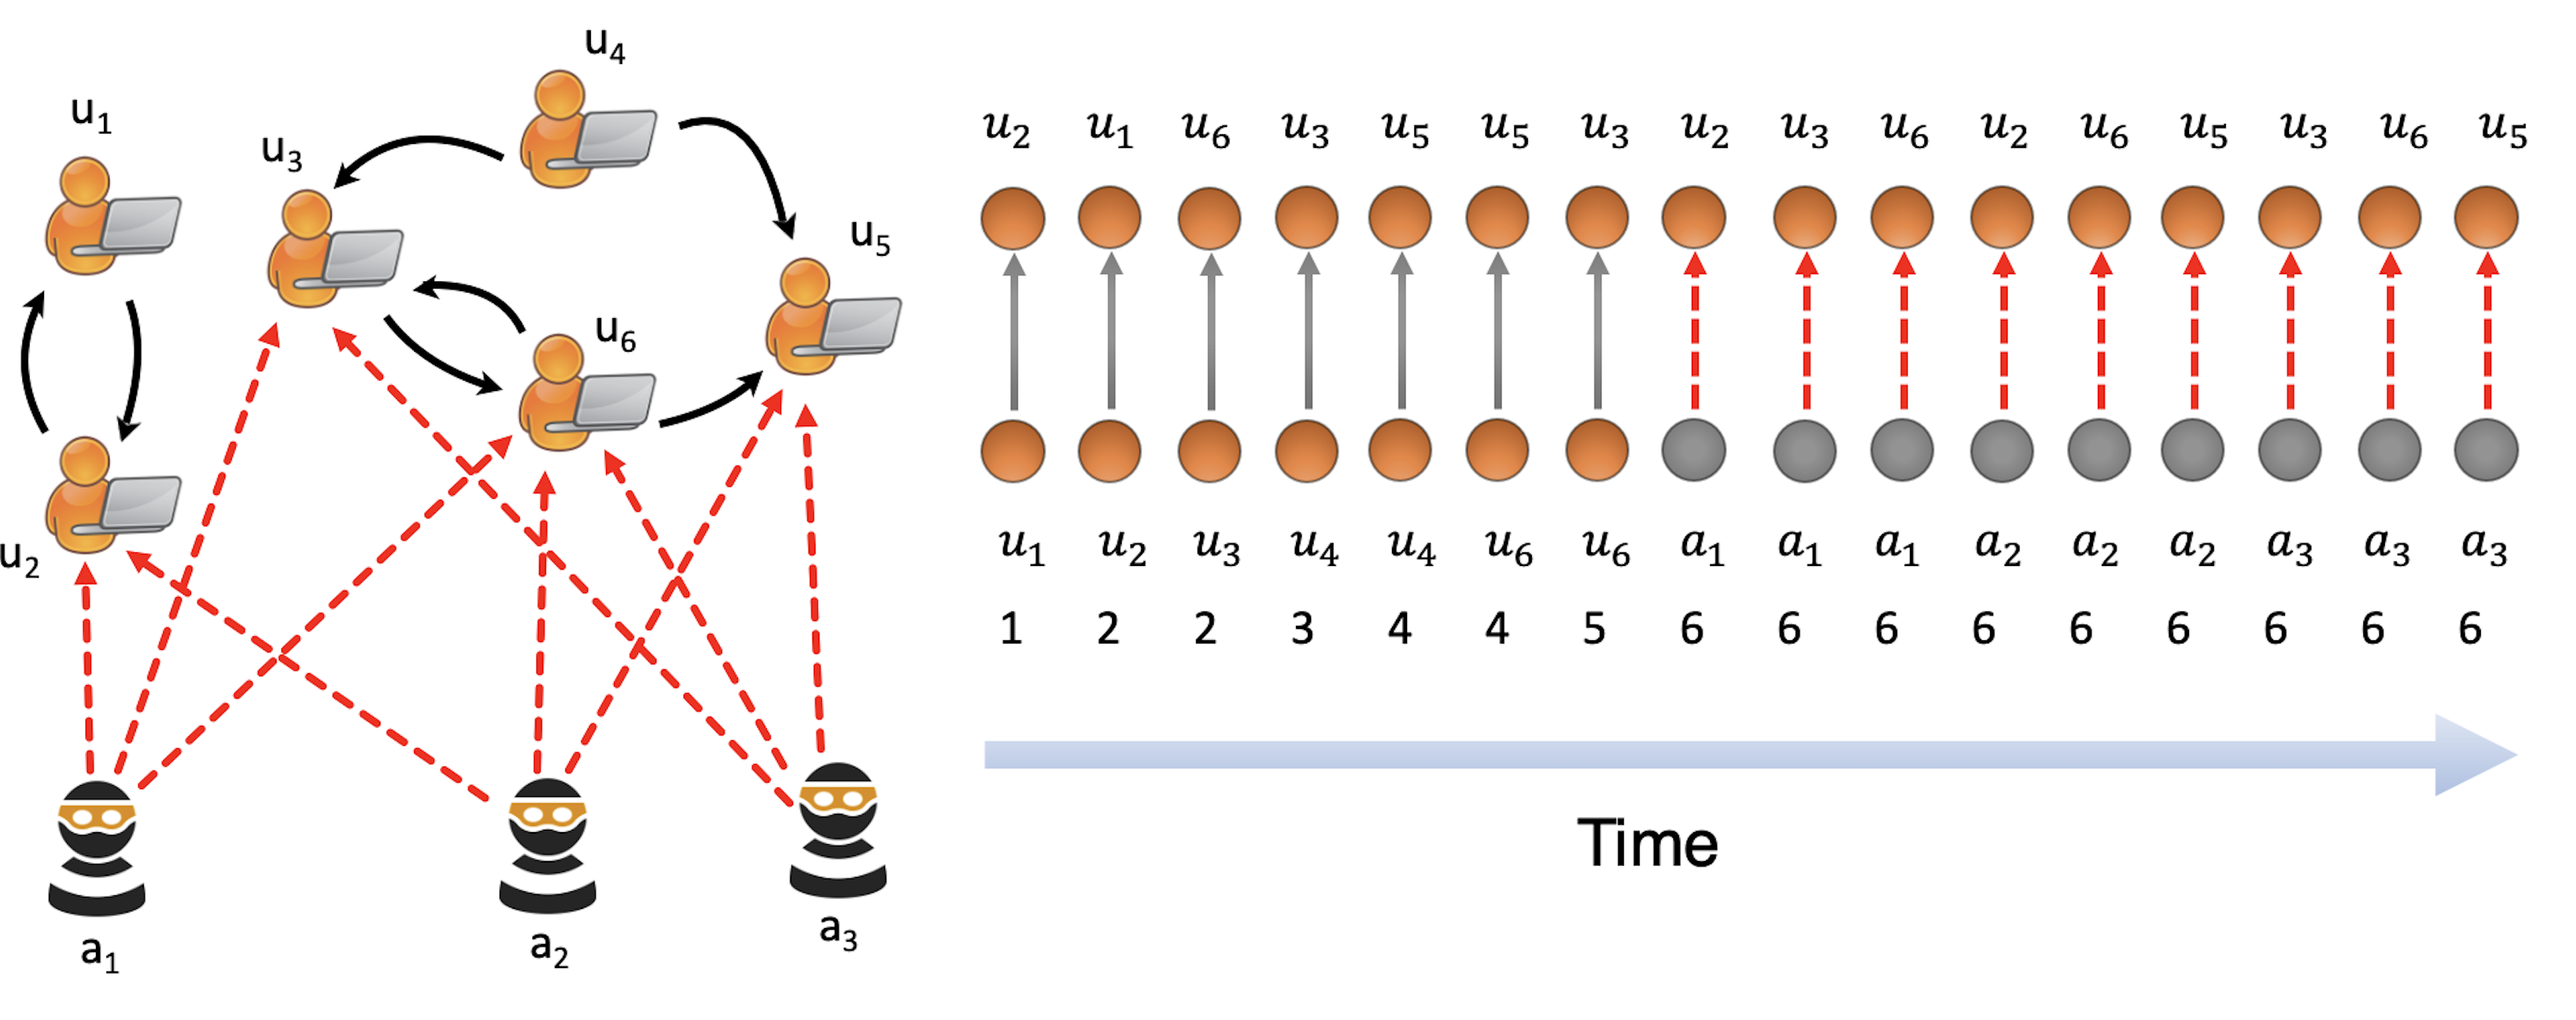
\includegraphics[width=1.0\textwidth]{figures/Intro.png}
    \caption{Minh họa cuộc tấn công mạng}
    \label{fig:2}
\end{figure}

Trong trường hợp này, các tác giả lập mô hình các nút(Node)
như máy tính xách tay, máy tính để bàn là
đỉnh của đồ thị, và một kết nối giữa chúng như là một cạnh(Edge).

Các sự kiện gian lận hoặc bất thường trong nhiều ứng dụng xảy ra trong các cụm vi mô(Microcluster) hoặc
đột nhiên đến các nhóm có cạnh giống nhau đáng ngờ, ví dụ: tấn công từ chối dịch vụ(Dos)
trong dữ liệu lưu lượng mạng. Các phương thức hiện có xử lý các luồng cạnh trong
một cách trực tuyến nhằm mục đích phát hiện các cạnh bất ngờ riêng lẻ, không phải các cụm vi mô và
do đó có thể bỏ lỡ một lượng lớn hoạt động đáng ngờ.


Thuật toán MIDAS sử dụng bản phác thảo đếm tối thiểu (CMS) để đếm số lần xuất hiện trong mỗi
dấu thời gian, sau đó sử dụng kiểm tra chi bình phương để đánh giá mức độ sai lệch và
tạo ra một số điểm đại diện cho sự bất thường. Điểm càng cao thì độ bất thường
của cạnh càng lớn. Phương pháp được đề xuất sử dụng bộ nhớ không đổi và
có độ phức tạp thời gian không đổi khi xử lý từng cạnh. Ngoài ra, bằng cách sử dụng một nguyên tắc
khuôn khổ thử nghiệm giả thuyết, MIDAS cung cấp các giới hạn lý thuyết về giả thuyết
xác suất dương mà những phương pháp tương tự khác
(\cite{related1},\cite{related2}) không cung cấp.

Hình \ref{fig:2} minh họa cách MIDAS tính điểm bất thường:
\begin{figure}[H]
    \centering
    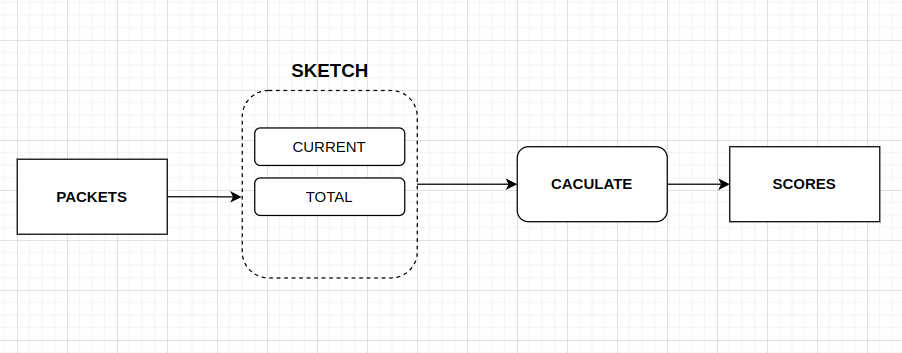
\includegraphics[width=1.0\textwidth]{figures/midas.png}
    \caption{Sơ đồ hoạt động MIDAS}
    \label{fig:3}
\end{figure}

Trong đó:
\begin{itemize}
    \item PACKETS: danh sách các gói tin mô phỏng một mạng thực.
    \item SKETCH: duyệt qua các gói tin và sử dụng CMS để ước lượng
          số lần xuất hiện của từng cạnh trong cùng thời điểm và trong toàn
          bộ thời gian chạy.
          \begin{itemize}
              \item CURRENT: đếm số lượng cạnh trong thời điểm hiện tại.
              \item TOTAL : đếm tổng số cạnh từ khi băt đầu theo dõi.
          \end{itemize}
    \item CALCULATE: tính toán điểm bất thường cho từng gói tin bằng kiểm định giả thiết Chi-Square để xác định sự tương quan giữa các mạng.
    \item SCORES: điểm bất thường của từng gói tin.
\end{itemize}

\RestyleAlgo{ruled}

%% This is needed if you want to add comments in
%% your algorithm with \Comment
\SetKwComment{Comment}{/* }{ */}

\begin{algorithm}[H]
    \caption{MIDAS: Streaming Anomaly Scoring}\label{alg:one}
    \KwData{Stream of graph edges over time}
    \KwOut{Anomaly scores per edge}
    $\triangleright$ \textbf{ Initialize CMS data structures:}\\
    Initialize CMS for total count $s_{uv}$ and current count $a_{av}$\\
    \While{$new\ edge\ e = (u, v, t)\ is\ received:$} {
        $\triangleright$  \textbf{Update Counts:}\\
        Update CMS data structures for the new edge $uv$\\
        $\triangleright$  \textbf{Query Counts:}\\
        Retrieve updated counts $\hat{s}_{uv}$ and $\hat{a}_{uv}$\\
        $\triangleright$  \textbf{Anomaly Score:}\\
        \textbf{output} score$(u,v,t)$ = $(\hat{a}_{uv} - \frac{\hat{s}_{uv}}{t})^2(\frac{t^2}{\hat{s}_{uv}(t-1)})$
    }
\end{algorithm}


\textbf{Algorithm \ref*{alg:one}} mô tả cách hoạt động của MIDAS, CMS được xóa sau mỗi lần thay đổi dấu thời gian. Tuy nhiên, một số bất thường vẫn tồn tại trong nhiều
dấu thời gian. Các tác giả của MIDAS đã đề xuất một biến thể được gọi là MIDAS-R có thể  duy trì
số lượng một phần của dấu thời gian trước đó cho phép tiếp theo
thuật toán để nhanh chóng tạo ra điểm cao khi cạnh xuất hiện trở lại. Nó cũng cũng coi các nút nguồn và đích là thông tin bổ sung
giúp xác định các cạnh bất thường.



\subsection{Thuật toán MIDAS-R}

Phần này mô tả cách tiếp cận của MIDAS-R\cite{midasr}, phương pháp này xem
xét các cạnh liên quan: nghĩa là, nó nhằm mục đích nhóm các cạnh gần nhau lại với nhau, hoặc
theo thời gian hoặc không gian.


\textbf{Quan hệ tạm thời:} Thay vì chỉ đếm các cạnh trong cùng một khoảng thời gian
(như đã làm ở MIDAS), các cạnh trong
quá khứ gần đây cũng sẽ được tính vào dấu thời gian hiện tại, nhưng được sửa đổi bằng cách giảm
cân nặng. Một cách đơn giản và hiệu quả để thực hiện việc này bằng cấu trúc dữ liệu CMS
như sau: vào cuối mỗi lần đánh dấu, thay vì đặt lại cấu trúc dữ liệu CMS
đối với $a_{uv}$, ta sẽ chia tỷ lệ tất cả số lượng của nó theo một phân số cố định $\alpha \in (0, 1)$. Điều này cho phép các cạnh trong quá khứ
để tính vào dấu tích thời gian hiện tại, với trọng số giảm dần. Lưu ý rằng
không xem xét 0 hoặc 1, vì 0 xóa tất cả các giá trị trước đó khi dấu thời gian thay đổi
và do đó không bao gồm bất kỳ hiệu ứng tạm thời nào; và 1 không chia tỷ lệ dữ liệu CMS
cấu trúc ở tất cả.

\textbf{Quan hệ không gian:} Nắm bắt các nhóm lớn không gian gần đó
các cạnh: ví dụ: một địa chỉ IP nguồn duy nhất đột nhiên tạo ra một số lượng lớn các cạnh
đến nhiều đích hoặc một nhóm nhỏ các nút đột nhiên tạo ra một
số lượng lớn các cạnh giữa chúng. Một trực giác đơn giản là ở một trong hai
hai trường hợp này, quan sát các nút có sự xuất hiện đột ngột của một lượng lớn
số cạnh. Do đó, chúng ta có thể sử dụng cấu trúc dữ liệu CMS để theo dõi cạnh
đếm như trước, ngoại trừ đếm tất cả các cạnh liền kề với bất kỳ nút u. Cụ thể,
tạo bộ đếm CMS cho $\hat{a}_u$ và $\hat{s}_u$ để tính gần đúng số lượng cạnh hiện tại và tổng số
liền kề với nút $u$. Với mỗi cạnh tới $(u,v)$, chúng ta có thể tính toán ba
điểm bất thường: một cho cạnh $(u,v)$, như trong thuật toán trước đây; một cho nút nguồn
$u$ và một cho nút đích $v$. Cuối cùng là kết hợp ba điểm bằng cách
lấy giá trị lớn nhất của chúng.


Hình \ref{fig:2} minh họa cách MIDAS-R tính điểm bất thường:

\begin{figure}[H]
    \centering
    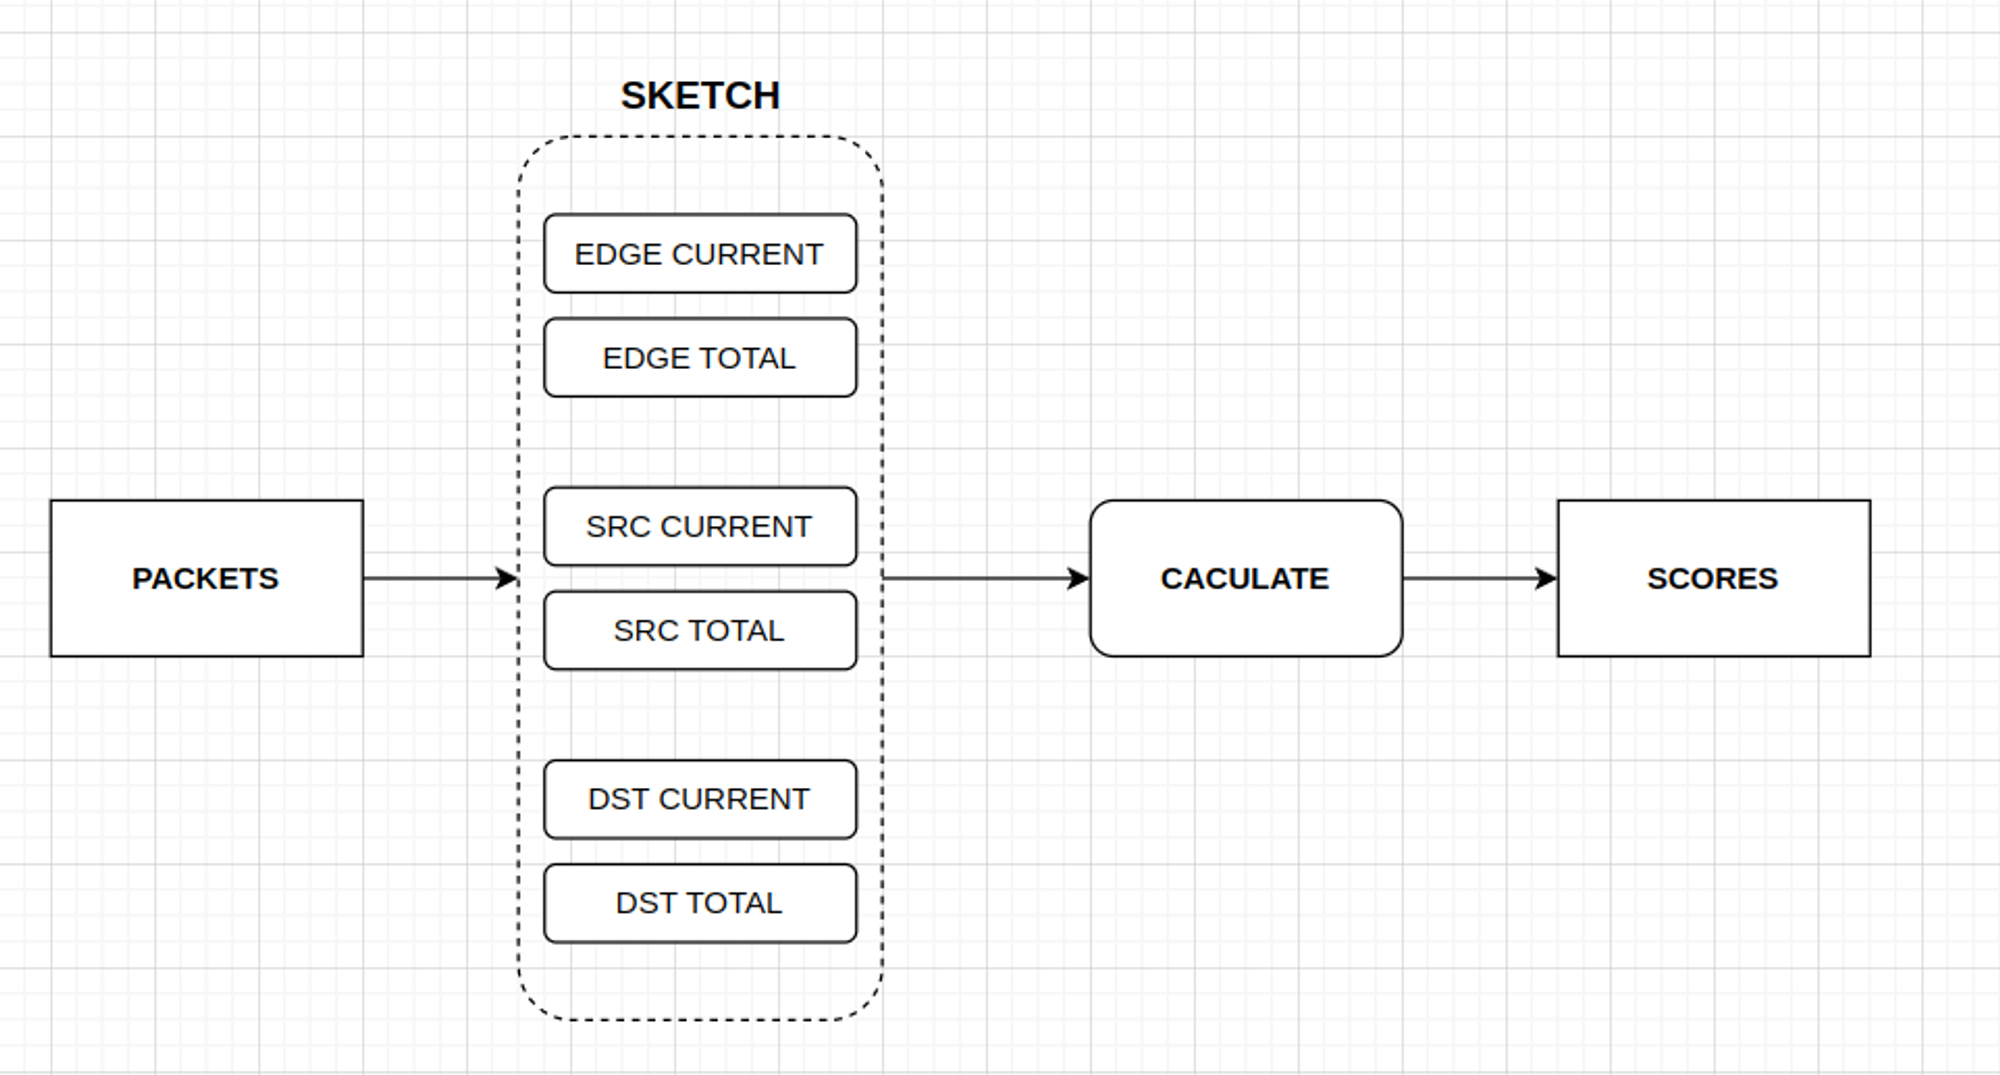
\includegraphics[width=1.0\textwidth]{figures/midasr.png}
    \caption{Sơ đồ hoạt động của MIDAS-R}
    \label{fig:4}
\end{figure}

Các khối trong hình \ref{fig:4} hoàn toàn tương tự như trong MIDAS được đề cập ở hình \ref{fig:3},
nhưng bổ sung thêm 4 khối:
\begin{itemize}
    \item SRC CURRENT: đếm số lượng nút nguồn hiện tại.
    \item SRC TOTAL: đếm tổng số nút nguồn từ khi bắt đầu theo dõi.
    \item DST CURRENT: đếm số lượng nút đích hiện tại.
    \item DST TOTAL: đếm tổng số nút đích từ khi băt đầu theo dõi.
\end{itemize}

Hoạt động của MIDAS-R được mô tả trong \textbf{Algorithm \ref*{alg:two}} dưới đây:

\begin{algorithm}[H]
    % with line numbers from second line
    \caption{MIDAS-R: Incorporating Relations}\label{alg:two}
    \KwData{Stream of graph edges over time}
    \KwOut{Anomaly scores per edge}
    $\triangleright$ \textbf{ Initialize CMS data structures:}\\
    Initialize CMS for total count $s_{uv}$ and current count $a_{uv}$\\
    Initialize CMS for total count $s_{u},s_{v}$ and current count $a_{u},a_{v}$\\
    \While{$new\ edge\ e = (u, v, t)\ is\ received:$} {
        $\triangleright$  \textbf{Update Counts:}\\
        Update CMS data structures for the new edge $uv$, source node $u$ and destination node $v$\\
        $\triangleright$  \textbf{Query Counts:}\\
        Retrieve updated counts $\hat{s}_{uv}$ and $\hat{a}_{uv}$\\
        Retrieve updated counts $\hat{s}_{u}, \hat{s}_{v}$ and $\hat{a}_{u}, \hat{a}_{v}$\\
        $\triangleright$  \textbf{Compute Edge Score:}\\
        score$((u,v,t))$ = $(\hat{a}_{uv} - \frac{\hat{s}_{uv}}{t})^2(\frac{t^2}{\hat{s}_{uv}(t-1)})$\\
        $\triangleright$  \textbf{Compute Node Scores:}\\
        score$((u,t))$ = $(\hat{a}_{u} - \frac{\hat{s}_{u}}{t})^2(\frac{t^2}{\hat{s}_{uv}(t-1)})$\\
        score$((v,t))$ = $(\hat{a}_{v} - \frac{\hat{s}_{v}}{t})^2(\frac{t^2}{\hat{s}_{uv}(t-1)})$\\
        $\triangleright$  \textbf{Final Score:}\\
        \textbf{output} max\{score$(u,v,t)$, score$(u,t)$, score$(v,t)$\}
    }
\end{algorithm}

\pagebreak


\subsection{Đánh giá và nêu vấn đề}

Các tác giả của MIDAS đã tiến hành đo lường\cite{midas}, kết quả được
mô tả trong bảng sau:

\begin{table}[H]
    \centering
    \caption{Độ chính xác(độ lệch chuẩn)}\label{tab:accuracy}
    \begin{tblr}{
        width = \linewidth,
        colspec = {Q[125]Q[112]Q[112]Q[123]Q[229]Q[229]},
        cells = {c},
        hlines,
        vlines,
        }
        Dataset & {PEN\\miner} & {F-\\FADE} & {SEDAN\\SPOT} & MIDAS & MIDAS-R\\
        \textit{DARPA} & 0.8267 & 0.8451 & 0.6442 & 0.9042(0.0032) & \textbf{0.9514}(0.0012)\\
        \textit{CTU-13} & 0.6041 & 0.8028 & 0.6397 & 0.9079(0.0049) & \textbf{0.9703}(0.0009)\\
        {\textit{UNSW}\\\textit{-NB15}} & 0.7028 & 0.6858 & 0.7575 & 0.8843(0.0079) & \textbf{0.8952}(0.0028)
    \end{tblr}
\end{table}

\begin{table}[H]
    \centering
    \caption{Thời gian chạy}\label{tab:runtime}
    \begin{tblr}{
        width = \linewidth,
        colspec = {Q[125]Q[112]Q[112]Q[123]Q[229]Q[229]},
        cells = {c},
        hlines,
        vlines,
        }
        Dataset & {PEN\\miner} & {F-\\FADE} & {SEDAN\\SPOT} & MIDAS & MIDAS-R\\
        \textit{DARPA} & 20423s & 325.1s & 67.54s & \textbf{0.09}s & 0.30s\\
        \textit{CTU-13} & 10065s & 844.2s & 38.73s & \textbf{0.05}s & 0.21s\\
        {\textit{UNSW}\\\textit{-NB15}} & 12857s & 2267s & 48.03s & \textbf{0.06}s & 0.15s
    \end{tblr}
\end{table}


Từ các khái niệm và hai bảng nêu trên, có thể đưa ra nhưng ưu diểm sau của MIDAS-R:
\begin{itemize}
    \item Có độ chính xác vượt trội so với các thuật toán khác.
    \item Chỉ cần sử dụng dữ liệu địa chỉ IP và dấu thời gian để phát hiện các bất thường
          thay vì cần rất nhiều trường như trong các phương pháp dựa trên học máy, thống kê, tri thức...
    \item Thời gian chạy nhanh hơn nhiều so với những thuật toán còn lại(trừ MIDAS).
    \item Không tiêu thụ thêm bộ nhớ trong thời gian chạy.
\end{itemize}

Tuy nhiên, MIDAS-R còn tồn tại các vấn đề sau:
\begin{itemize}
    \item Thời gian xử lý chậm hơn MIDAS tới 3 lần.
    \item Chỉ có thể xử lý tuần tự tất cả các gói tin, điều này là không
          khả thi trong môi trường có lưu lượng mạng lớn và thay đổi đột ngột,
          nhất là trong giai đoạn bùng nổ truy cập Internet như hiện nay.
\end{itemize}


\section{Nội dung đồ án}

\subsection{Mục tiêu và phương pháp}
\begin{itemize}
    \item Mục tiêu:
          \begin{itemize}
              \item Cải thiện hiệu năng thuật toán MIDAS-R
                    ít nhất 40\% so với thuật toán ban đầu trong khi vẫn đảm bảo độ chính xác.
              \item Bổ sung khả năng thích ứng trong điều kiện
                    lưu lượng mạng thay đổi theo thời gian.
          \end{itemize}

    \item Phương pháp: Để giải quyết vấn đề này,
          đầu tiên cần tiến hành phân tích điểm nghẽn hiệu năng tại các bước xử lý trong MIDAS-R và
          đưa ra các cách cải tiến phù hợp.
\end{itemize}


\begin{tcolorbox}
    \textbf{Note:} Trong khuôn khổ đồ án này, em chỉ tập trung cải tiến thuật toán MIDAS-R.
    Tuy nhiên các phương pháp cải thiện được đề xuất hoàn toàn có thể áp dụng cho các thuật toán MIDAS
    và các biến thể của nó.
\end{tcolorbox}

\subsection{Phạm vi của đồ án}
\begin{itemize}
    \item  Toàn bộ việc triển khai thuật toán MIDAS-R được thực hiện hoàn toàn trên máy tính.
    \item Dữ liệu tấn công đã được tiền xử lý dưới dạng file CSV thu thập từ các
          các tổ chức an ninh mạng.
\end{itemize}

\subsection{Phần mềm và công cụ}

\begin{itemize}
    \item Ngôn ngữ lập trình C được sử dụng để triển khai thuật toán.
    \item Ngôn ngữ script Python dùng cho tổng hợp và trực quan hóa số liệu.
    \item Công cụ Make để tự động hóa quá trình biên dịch và liên kết.
    \item Đo lường hiệu suất: perf, flamegraph.
    \item Môi trường triển khai trên hệ điều hành Linux.
\end{itemize}
\chapter{PHÂN TÍCH VÀ CẢI THIỆN THUẬT TOÁN}

\section{Đo lường, phân tích các nút thắt cổ chai và đề xuất cải tiến}

\section{Bản phác thảo NitroSketch}

\section{Tạo hàm băm hiệu quả}

\section{Các phương pháp khác}
\chapter{ĐO LƯỜNG, ĐÁNH GIÁ VÀ KẾT LUẬN}

\section{Chuẩn bị}
\section{Độ chính xác}
\section{Hiệu năng}
\section{Kết luận}

\singlespacing

\clearpage
\bibliography{refs}
\addcontentsline{toc}{chapter}{References}
\bibliographystyle{plainnat}

\begin{appendices}
\chapter{This is title of appendix A}
\chapter{This is title of appendix B}
\end{appendices}

\end{document}
